%% =====================================================================
%% Econometric Analysis of Firm Data (KAN-CEAPV2505U) -- Final project
%% Manager gender and technology adoption in Peruvian firms, 2010-2023
%%
%% Compile:  latexmk -pdf main.tex      (or: pdflatex, bibtex, pdflatex x2)
%% Every table in tables/ and the figure in figures/ is written by the
%% R notebook peru_gender_technology_panel.Rmd. Re-run the notebook to
%% update the numbers; do not edit the table files by hand.
%% =====================================================================
\documentclass[11pt,a4paper]{article}

\usepackage[utf8]{inputenc}
\usepackage{fontawesome5}
\IfFileExists{lmodern.sty}{\usepackage[T1]{fontenc}\usepackage{lmodern}}{}
\usepackage[margin=2.5cm]{geometry}
\usepackage{amsmath,amssymb}
\usepackage{booktabs,threeparttable,tabularx}
\usepackage{graphicx}
\usepackage[font=small,labelfont=bf]{caption}
\usepackage{pdfpages}
\usepackage[round,authoryear]{natbib}
\usepackage[hidelinks]{hyperref}
\setlength{\parskip}{0.35em}
\renewcommand{\arraystretch}{1.05}

\newcommand{\tabnotes}[1]{\begin{tablenotes}[flushleft]\footnotesize\item #1\end{tablenotes}}

% ---- edit these
\newcommand{\studentname}{Carla de Erausquin}
\newcommand{\studentno}{185899}

\begin{document}


\begin{center}
{\Large\bfseries Manager Gender and Technology Adoption in Peruvian Firms, 2010--2023:\\[0.2em] Evidence from an Unbalanced Firm Panel}\\[1em]
{\large \studentname\ (\studentno)}\\[0.3em]
KAN-CEAPV2505U Econometric Analysis of Firm Data \quad$\cdot$\quad Copenhagen Business School\\[0.5em]
\faGithub\ \href{https://github.com/deercarla/econometric-analysis-of-firm-data}{\texttt{GitHub Repository}}\\[0.3em]
\today
\end{center}


%% =====================================================================
\section{Introduction}
%% =====================================================================

Firms led by women differ from firms led by men in many ways: female-owned firms tend to be smaller \citep{bruhn2009} and female managers are more prevalent in retail \citep{amin2014}. Whether female-led firms are also less likely to adopt technology is therefore hard to answer with a simple comparison, because a raw gap mixes the role of manager gender with the role of size, sector and many unobserved firm traits. Timing adds a second question. Over the last fifteen years digital tools became cheaper and more widespread, and the COVID-19 pandemic made online presence more valuable for all firms. Evidence from the World Bank's COVID-19 follow-up surveys suggests that female-owned firms were hit harder by the crisis but moved activities online about as often as male-owned firms \citep{hyland2021}. Whether the gender gap in technology adoption has changed over time is therefore an open empirical question.

This project asks one question: \emph{are Peruvian formal firms with a female top manager less likely to adopt technology once unobserved, time-constant firm differences are taken into account, and how did this gap evolve between 2010, 2017 and 2023?} Technology adoption is measured by two binary outcomes: whether the firm has its own website (digital presence) and whether it holds an internationally recognised quality certification (adoption of formal standards). I use three waves of the World Bank Enterprise Surveys for Peru, which I link into an unbalanced panel of 2,258 firms. The 2023 wave is the first one after the pandemic, but because all firms were exposed to it, the design compares gender gaps across waves rather than identifying an effect of COVID-19.

The analysis focuses on one econometric problem, unobserved firm heterogeneity in an unbalanced panel, and treats it in depth. I start from a pooled linear probability model and check its functional form with a probit model. I then compare pooled OLS, random effects (RE) and fixed effects (FE), use the Mundlak test to ask whether the firm effects are correlated with the regressors, and, because the panel is unbalanced, test whether the way firms enter and leave the panel is related to the outcomes.

Three findings stand out. First, for websites, female-led firms were about 6 percentage points (pp) less likely to have one before the pandemic, conditional on observable characteristics. RE and FE point in the same direction, although FE is imprecise. The gap narrowed over time, but most of the narrowing appears to have happened between 2010 and 2017, not after the pandemic. Second, for certification, the pooled models show a significant gap of about 5--6 pp in 2023, but it weakens substantially when the analysis is restricted to firms observed more than once; on that common sample, pooled OLS, RE and FE give similar and imprecise estimates. Sample composition, rather than the choice of estimator, matters most for this result. Third, the Mundlak test rejects the RE restrictions for certification, but the strongest evidence concerns firm size, and the gender averages are not significant even jointly, which shows that a joint specification test can reject even when the coefficients of interest are similar across estimators.

%% =====================================================================
\section{Data}
%% =====================================================================

\subsection{Source and panel construction}

The World Bank Enterprise Surveys interview formal, private, non-agricultural firms with at least five employees, sampled by size, sector and region. I use two files: the Peru 2006--2017 panel, which contains the 2010 wave \citep{wbes0617}, and the Peru 2017--2023 panel file, which contains the 2017 wave and the 2023 survey \citep{wbes2023}. Both files contain the same 2017 survey with the same firm identifier, so the panel is linked through the 2017 wave: a firm observed in 2017 receives the same key in both files, and a firm observed only in 2010 or only in 2023 receives a file-specific key. This rule cannot link a firm observed in 2010 and 2023 but not in 2017, so I checked whether such firms exist in the source data. The World Bank's panel indicator in the 2017--2023 file classifies every 2023 firm either as newly sampled in 2023 (629 firms) or as re-interviewed from 2017 (358 firms); the 2023 panel component was drawn from the 2017 sample, and no 2023 firm carries an identifier from the 2010 survey. The survey design therefore records no firm as observed in 2010 and 2023 without 2017, and every repeated firm in the linked panel is observed in consecutive waves. This does not rule out that the same establishment was independently sampled in 2010 and again as a new firm in 2023; such a firm could not be identified with the available identifiers and appears as two firms.

\begin{table}[t]
\centering\footnotesize
\begin{threeparttable}
\caption{Structure of the linked panel}\label{tab:panel}
\begin{tabular}{lrrrr}
\toprule
Observed in & Firms & 2010 & 2017 & 2023 \\
\midrule
2010 only & 626 & $\times$ & & \\
2017 only & 414 & & $\times$ & \\
2023 only & 629 & & & $\times$ \\
2010 and 2017 & 231 & $\times$ & $\times$ & \\
2017 and 2023 & 215 & & $\times$ & $\times$ \\
2010, 2017 and 2023 & 143 & $\times$ & $\times$ & $\times$ \\
\midrule
Total firms & 2,258 & & & \\
Firm-year observations & 2,990 & 1,000 & 1,003 & 987 \\
\bottomrule
\end{tabular}
\tabnotes{Firms are linked through the 2017 survey identifier, which is identical in both source files. 589 firms are observed in at least two waves.}
\end{threeparttable}
\end{table}

Table~\ref{tab:panel} shows the result. The panel is strongly unbalanced: 1,669 of the 2,258 firms are observed only once, and only 589 firms, with about 1,290 observations, provide variation \emph{within} firms. This distinction matters throughout the paper. Pooled OLS and RE use all 2,990 observations, whereas FE is identified only by the repeated firms. The unbalancedness has two sources: the survey adds new firms in each wave by design (refreshment samples), and some earlier firms are not re-interviewed because they closed, refused or could not be contacted (attrition). Section~\ref{sec:sel} discusses when each source threatens the estimates.

\subsection{Variables}

The key regressor $F_{it}$ equals one if the top manager is a woman. The outcomes are dummies for having an own website and for holding an internationally recognised quality certification. Both describe the firm's status at the interview, so the 2023 values reflect the situation after the pandemic. The time-varying controls are log permanent full-time employees, the top manager's years of experience in the sector, exporter status (direct exports $\geq$10\% of sales) and foreign ownership ($\geq$10\%). Pooled OLS and RE also include three broad sectors and five regions. Sector is coded differently in 2010 (ISIC two-digit codes) and in 2017--2023 (sampling sector), so I use three categories that can be built consistently: manufacturing, retail and other services. I tabulated the raw sector and region codes by wave before classifying them; all codes are valid categories, so no missing or unexpected code is assigned to ``other services''. For 41 of the 589 repeated firms the recorded sector differs between waves, and for 4 the region; Section~\ref{sec:sector} discusses what this implies. Answers coded as ``don't know'', refused or not applicable are set to missing in all variables. The estimation samples are 2,955 observations (2,239 firms) for website and 2,875 observations (2,185 firms) for certification.

Two variables are deliberately left out. Firm age equals the survey year minus the founding year; with year dummies the founding year is time-constant, so age cannot be separated from the firm and year effects in FE, and I omit it in all models to keep them comparable. Membership of a larger firm falls from about 20\% of firms in 2017 to about 1\% in 2023 (Table~\ref{tab:desc}), which points to a change in the questionnaire rather than in the firms; inside FE it would create artificial within-firm changes, so it is not used as a control.

\begin{table}[t]
\centering\footnotesize
\setlength{\tabcolsep}{4pt}
\begin{threeparttable}
\caption{Means by survey wave and gender of the top manager}\label{tab:desc}
\begin{tabular}{lcccccc}
\toprule
 & \multicolumn{2}{c}{2010} & \multicolumn{2}{c}{2017} & \multicolumn{2}{c}{2023} \\
\cmidrule(lr){2-3}\cmidrule(lr){4-5}\cmidrule(lr){6-7}
 & Male-led & Female-led & Male-led & Female-led & Male-led & Female-led \\
\midrule
Own website & 0.678 & 0.529 & 0.692 & 0.599 & 0.797 & 0.757 \\
Quality certification & 0.262 & 0.202 & 0.224 & 0.109 & 0.225 & 0.127 \\
\addlinespace
Employees (permanent full-time) & 195.3 & 128.6 & 172.2 & 95.2 & 104.0 & 95.6 \\
Manager experience (years) & 22.2 & 22.4 & 24.6 & 22.8 & 23.8 & 21.9 \\
Exporter ($\geq$10\% of sales) & 0.230 & 0.235 & 0.173 & 0.155 & 0.145 & 0.121 \\
Foreign owned ($\geq$10\%) & 0.125 & 0.067 & 0.099 & 0.048 & 0.092 & 0.074 \\
Part of larger firm & 0.203 & 0.160 & 0.248 & 0.171 & 0.012 & 0.000 \\
Manufacturing & 0.759 & 0.765 & 0.564 & 0.545 & 0.473 & 0.386 \\
Retail & 0.102 & 0.118 & 0.167 & 0.209 & 0.145 & 0.223 \\
\midrule
Firms & 880 & 119 & 816 & 187 & 772 & 215 \\
\bottomrule
\end{tabular}

\tabnotes{Unweighted means. Employees and experience in levels, other rows are shares.}
\end{threeparttable}
\end{table}

\subsection{Sector and region changes within firms}\label{sec:sector}

Fixed effects remove only characteristics that are constant over time, so a change in a firm's recorded sector matters for the estimator comparison. All 41 sector changes occur between 2017 and 2023, where both waves use the same sampling-sector variable; none occurs between 2010 and 2017, where the coding switches from ISIC codes to sampling sectors, so the harmonisation of the 2010 codes is not their source. More than half (23) are moves between retail and other services, a boundary that is easy to assign differently, for example for firms that both sell and repair goods. Whether the changes reflect real changes in activity or a different sector assignment in the 2023 sample frame cannot be determined from the data. The two readings have different implications. If the changes are measurement differences, sector is effectively time-constant and correctly absorbed by the firm effect in FE. If they are real, sector is time-varying, and leaving it out of FE while including it in pooled OLS and RE makes the estimators condition on different information. I therefore keep sector and region as wave-specific controls in pooled OLS and RE, and check whether adding them to FE changes the results (Section~\ref{sec:rob}).

\subsection{Descriptive patterns}

Table~\ref{tab:desc} and Figure~\ref{fig:outcomes} show that female-led firms are less likely to have a website and a certificate in every wave, and that they are smaller and less often foreign-owned. The raw website gap narrows from 14.9 pp in 2010 and 9.3 pp in 2017 to 4.0 pp in 2023 (Welch $t$-tests: $p=0.003$, $0.019$ and $0.23$). The raw certification gap is 6.0 pp in 2010 ($p=0.14$), 11.5 pp in 2017 and 9.9 pp in 2023 (both $p<0.001$). Each wave in Figure~\ref{fig:outcomes} is a full cross-section, so the changes between waves mix changes within firms with changes in which firms are sampled. Because female-led firms also differ in size and sector, these raw gaps cannot be attributed to manager gender, which is why the analysis turns to regression and panel methods.

\begin{figure}[t]
\centering
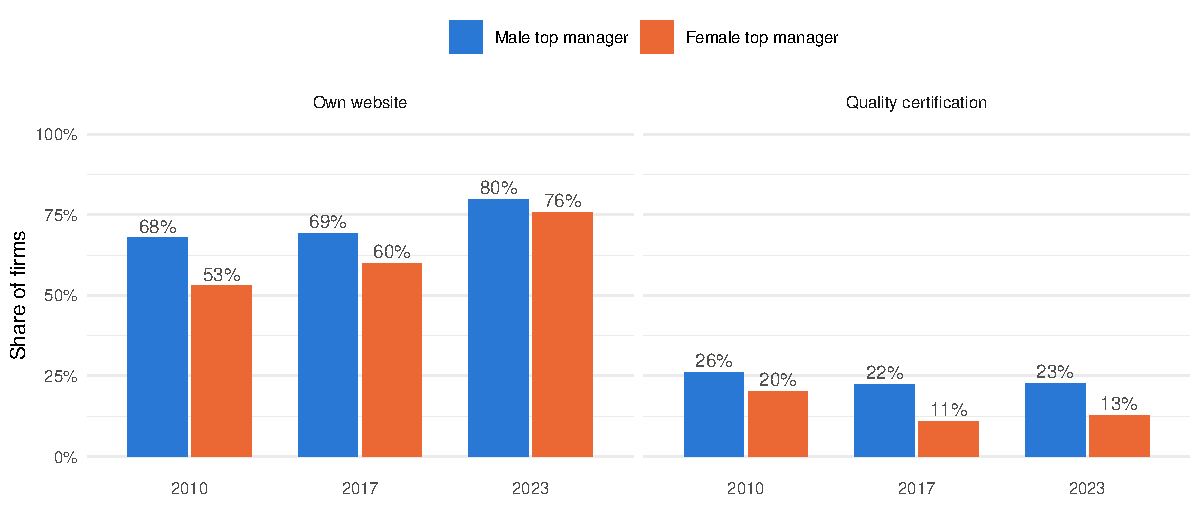
\includegraphics[width=\textwidth]{figures/fig1_outcomes.pdf}
\caption{Share of firms with each outcome, by survey wave and gender of the top manager. Unweighted; each wave is the full cross-section.}\label{fig:outcomes}
\end{figure}

%% =====================================================================
\section{Econometric approach}
%% =====================================================================

\subsection{The linear probability model and pooled OLS}

The baseline model for outcome $y_{it}\in\{0,1\}$ of firm $i$ in wave $t$ is
\begin{equation}\label{eq:lpm}
y_{it} = \beta_0 + \beta_1 F_{it} + \beta_3 \,(F_{it}\times D^{23}_t) + \delta_1 D^{17}_t + \delta_2 D^{23}_t + \mathbf{x}_{it}'\boldsymbol\gamma + v_{it}
\equiv \mathbf z_{it}'\boldsymbol\beta + v_{it},
\end{equation}
where $D^{17}_t$ and $D^{23}_t$ are wave dummies, $\mathbf{x}_{it}$ contains the controls and $\mathbf z_{it}$ collects all regressors. Because $y$ is binary, $E(y_{it}\mid\mathbf z_{it})=P(y_{it}=1\mid\mathbf z_{it})$, so each coefficient is a change in probability: this is the linear probability model (LPM). $\beta_1$ is the female--male gap before the pandemic (2010 and 2017 pooled), $\beta_1+\beta_3$ the gap in 2023 and $\beta_3$ the change in the gap. Pooling 2010 and 2017 is a restriction; Section~\ref{sec:rob} relaxes it.

Estimating \eqref{eq:lpm} by OLS on all observations (pooled OLS) is consistent if $E(v_{it}\mid\mathbf z_{it})=0$, that is, if no omitted factor is correlated with manager gender, the wave dummies or the controls. Two features of the data determine the inference \citep[ch.~8, 13]{wooldridge2025}. First, the LPM error is heteroskedastic by construction: $\operatorname{Var}(v_{it}\mid\mathbf z_{it})=p(\mathbf z_{it})[1-p(\mathbf z_{it})]$, which depends on the regressors. Second, the same firm can appear up to three times, and its errors are correlated across waves. I therefore use standard errors clustered by firm, which are robust to both problems. With about 2,900 observations, inference relies on asymptotic normality, so normally distributed errors are not required.

\paragraph{Probit check.} The LPM can predict probabilities outside $[0,1]$ and assumes constant partial effects. A probit model instead assumes a latent variable $y^*_{it}=\mathbf z_{it}'\boldsymbol\beta+e_{it}$ with $e_{it}\sim N(0,1)$ and $y_{it}=\mathbb 1[y^*_{it}>0]$, so that $P(y_{it}=1\mid\mathbf z_{it})=\Phi(\mathbf z_{it}'\boldsymbol\beta)$, and is estimated by maximum likelihood \citep[ch.~17]{wooldridge2025}. Its coefficients are not partial effects, because $\partial P/\partial z_j=\phi(\mathbf z'\boldsymbol\beta)\beta_j$ depends on all regressors. For the female dummy I compute the average partial effect (APE): the average over firms of the change in predicted probability when $F$ switches from 0 to 1, separately for the pre-pandemic waves and for 2023, and the difference between the two. The difference is computed on the probability scale because, in a nonlinear model, the coefficient on an interaction term is not the change in the effect. Standard errors come from a bootstrap that resamples whole firms (199 replications). The probit is used only as a check: if its APEs are close to the LPM coefficients, the conclusions do not depend on the linear functional form, and the LPM can be used in the panel models, where it is much easier to remove firm effects.

\subsection{Unobserved firm heterogeneity: pooled OLS, random effects and fixed effects}

Pooled OLS treats the error as a single term. In panel data it is natural to split it into a time-constant firm effect $a_i$ and an idiosyncratic error $u_{it}$:
\begin{equation}\label{eq:uem}
y_{it} = \beta_1 F_{it} + \beta_3 \,(F_{it}\times D^{23}_t) + \delta_1 D^{17}_t + \delta_2 D^{23}_t + \mathbf{x}_{it}'\boldsymbol\gamma + a_i + u_{it}.
\end{equation}
The firm effect $a_i$ contains everything about a firm that does not change over time and is not observed: management culture, market niche, the owner's networks, location. If $a_i$ is correlated with manager gender, both pooled OLS and RE are inconsistent (heterogeneity bias), however many observable controls are added \citep[ch.~13--14]{wooldridge2025}.

\paragraph{Random effects.} RE assumes that $a_i$ is uncorrelated with all regressors in all periods. Under this assumption pooled OLS is also consistent, but it is inefficient, because the composite error $a_i+u_{it}$ is serially correlated: $\operatorname{Cov}(a_i+u_{it},a_i+u_{is})=\sigma_a^2$ for $t\neq s$. RE is the feasible GLS estimator that accounts for this correlation. It amounts to pooled OLS on quasi-demeaned data, $y_{it}-\theta_i\bar y_i$ and $\mathbf z_{it}-\theta_i\bar{\mathbf z}_i$, with $\theta_i=1-\sqrt{\sigma_u^2/(\sigma_u^2+T_i\sigma_a^2)}$. In an unbalanced panel $\theta_i$ differs across firms because it depends on the number of waves $T_i$ in which firm $i$ is observed. RE lies between pooled OLS ($\theta_i=0$) and FE ($\theta_i=1$), and it can still estimate the effects of variables that do not vary within firms.

\paragraph{Fixed effects.} FE drops the assumption on $a_i$. It subtracts each firm's own average over the waves in which it is observed, $\ddot y_{it}=y_{it}-\bar y_i$, which removes $a_i$, and then applies pooled OLS to the demeaned data. FE allows any correlation between $a_i$ and the regressors. The price is that only variation \emph{within} firms is used. A firm observed once has $\ddot y_{it}=0$ and $\ddot{\mathbf z}_{it}=\mathbf 0$, so it contributes nothing, even though it is counted among the observations in the regression output; the effective FE sample is 1,293 observations from 577 firms for website and 1,252 observations from 562 firms for certification.

\paragraph{What FE identifies here.} The gender variables are measured contemporaneously, so it is worth being precise about which within-firm changes identify them. In the website sample, $\beta_1$ is identified by the 61 repeated firms whose top manager changes gender between waves (60 in the certification sample), and a change of manager may coincide with other changes in the firm. $\beta_3$ draws on the 70 firms (68) in which $F_{it}\times D^{23}_t$ changes; 53 (51) of them are led by a woman in every wave, so the interaction changes only because the 2023 wave arrives. Both estimates therefore rest on few firms and will be imprecise. Because a firm that changes manager can change both $F_{it}$ and $F_{it}\times D^{23}_t$, $\beta_3$ is not a before-and-after comparison of firms classified by their pre-pandemic manager. It measures how the within-firm association between \emph{current} manager gender and the outcome differs in 2023, and $\beta_1+\beta_3$ is a model-implied gender contrast in 2023, not a direct comparison of otherwise identical firms in that year. None of these coefficients is a causal effect of female leadership.

\paragraph{Assumptions behind FE in an unbalanced panel.} Following the lecture on unbalanced panels, FE requires (i) strict exogeneity, which now includes the selection indicators: $E(u_{it}\mid\mathbf z_{i1},\dots,\mathbf z_{iT},s_{i1},\dots,s_{iT},a_i)=0$; (ii) a rank condition, so that every regressor varies within firms in the observed waves, which is why firm age cannot be included and sector and region, which change for only a few firms, are left out of the main FE specification; and (iii) for the usual standard errors, homoskedastic and serially uncorrelated $u_{it}$. Condition (iii) fails for a binary outcome, so all FE inference uses standard errors clustered by firm, which are valid under arbitrary heteroskedasticity and serial correlation within firms. Condition (i) is the one that cannot be taken for granted, because it requires $u_{it}$ to be unrelated to the regressors in \emph{every} wave, including future ones. In this application the most plausible failure runs through manager turnover: a firm that unexpectedly falls behind in technology adoption may appoint a different top manager by the next wave, so that today's shock predicts tomorrow's $F_{i,t+1}$. FE would then attribute part of the shock to manager gender. One implication can be checked: adding $F_{i,t+1}$, manager gender in the \emph{next survey wave}, to the FE regression should give a zero coefficient \citep[ch.~10]{wooldridge2010}. This is a diagnostic of one implication, not a test of the assumption itself, and in a three-wave panel it has little power, because only firms observed in all three waves have two observations with a known lead. The selection part of condition (i) is tested in Section~\ref{sec:sel}.

\paragraph{Why FE rather than first differences, and why a linear model?} First differencing also removes $a_i$. Because every repeated firm in this panel is observed in consecutive waves, the two estimators coincide for the 446 firms observed exactly twice and differ only for the 143 firms observed three times. The textbook benchmark is that FE is efficient when the $u_{it}$ are serially uncorrelated and first differencing when they follow a random walk \citep[ch.~14]{wooldridge2025}. These results assume homoskedastic errors, which a binary outcome does not satisfy, so they only serve as a guide; with gaps of six and seven years between waves, serially uncorrelated shocks are the more plausible benchmark, and I use FE. Inference is cluster-robust in either case. The panel models are linear because the LPM allows $a_i$ to be removed by demeaning. In a probit, including a dummy for each firm would give inconsistent estimates with at most three observations per firm (the incidental parameters problem), and the probit check suggests that little is lost by using the linear model.

\subsection{Testing the RE assumption: the Mundlak approach}

RE is consistent and more efficient if $a_i$ is uncorrelated with the regressors; FE is consistent either way. Following the course, I test this assumption with the Mundlak approach rather than the classical Hausman test, because it does not require RE to be fully efficient and can use cluster-robust standard errors. \citet{mundlak1978} models the firm effect as a function of the firm averages $\bar{\mathbf w}_i$ of the time-varying regressors, here $F_{it}$, $F_{it}\times D^{23}_t$ and the four time-varying controls:
\begin{equation}\label{eq:mundlak}
a_i=\bar{\mathbf w}_i'\boldsymbol\xi+\bar{\mathbf d}_i'\boldsymbol\lambda+c_i
\quad\Rightarrow\quad
y_{it}=\mathbf z_{it}'\boldsymbol\beta+\bar{\mathbf w}_i'\boldsymbol\xi+\bar{\mathbf d}_i'\boldsymbol\lambda+c_i+u_{it}.
\end{equation}
All averages are taken over the waves in which firm $i$ is observed. In an unbalanced panel the averages of the wave dummies, $\bar{\mathbf d}_i=(\bar D^{17}_i,\bar D^{23}_i)$, also differ across firms, because they record \emph{which} waves a firm is observed in; \citet{wooldridge2019} recommends including them so that the firm effect may depend on the observation pattern. They are included as controls and are not part of the tested restriction.

The approach also shows why the test compares two sources of variation. If $\bar{\mathbf w}_i$ and $\bar{\mathbf d}_i$ contain the averages of \emph{all} time-varying regressors in the specification, computed on the estimation sample, pooled OLS on \eqref{eq:mundlak} gives exactly the FE estimate of $\boldsymbol\beta$, because the averages absorb all variation between firms, and in a balanced panel $\hat{\boldsymbol\xi}$ equals the difference between the between-firm and the within-firm estimates. I verified this equivalence in the notebook: without sector and region, which change within some firms, pooled OLS with the averages reproduces the FE coefficients on $F_{it}$ and $F_{it}\times D^{23}_t$ to the fourth decimal. RE corresponds to $\boldsymbol\xi=\mathbf 0$: the between- and within-firm relationships are the same, and both can be pooled.

I estimate \eqref{eq:mundlak} by RE and test $H_0:\boldsymbol\xi=\mathbf 0$ with a cluster-robust Wald test, which is asymptotically $\chi^2_6$. A rejection is evidence against the RE restriction that $a_i$ is uncorrelated with the regressors, and favours FE, provided that FE's own assumptions hold. A non-rejection does not show that the restriction holds; it means that the data do not contradict it. Because the test is joint, a rejection says that \emph{some} regressor is correlated with $a_i$, not that manager gender is. The individual coefficients on $\bar F_i$ and on the average of $F_{it}\times D^{23}_t$ show whether the firm effect is related to manager gender in particular.

\subsection{Unbalanced panels and sample selection}\label{sec:sel}

Estimation with an unbalanced panel works mechanically as with a balanced one; the question is \emph{why} observations are missing \citep[sec.~19.9]{wooldridge2010}. Let $s_{it}=1$ if firm $i$ is observed in wave $t$. Missing observations cause no bias if selection is unrelated to the errors, as in a rotating panel where firms are added at random. Here the survey adds new firms by design, which is harmless, but it also loses firms that close, refuse or cannot be contacted. This attrition is a problem if it depends on the shocks $u_{it}$, for example if firms that had a bad year are less likely to be re-interviewed.

The FE estimator on the unbalanced panel is consistent if $s_{it}$ is unrelated to $u_{ir}$ for all $t$ and $r$, conditional on the regressors and $a_i$. Selection may be correlated with $a_i$ itself, since FE removes it: it is not a problem if, say, persistently better-managed firms are more likely to stay in the panel. RE requires more: $a_i$ must also be unrelated to selection. These conditions can be tested. Under strict exogeneity, selection in another period should not help explain $y_{it}$ once the regressors and $a_i$ are controlled for \citep{wooldridge2019}. I run three tests, each with a cluster-robust $t$-test:
\begin{itemize}
  \item \emph{FE with a lead:} add $s_{i,t+1}$ (observed in the \emph{next} wave); 2023 is lost. A significant coefficient means that firms that later drop out had different shocks, the case most directly related to attrition.
  \item \emph{FE with a lag:} add $s_{i,t-1}$ (observed in the \emph{previous} wave); 2010 is lost.
  \item \emph{RE with $T_i$:} add the number of waves observed, which is time-constant and cannot enter FE.
\end{itemize}
The indicators refer to the adjacent survey \emph{wave}, not the next calendar year: $s_{i,t+1}$ in 2010 equals one if the firm is observed in 2017, and so on. The lead regressions use 1,978 (website) and 1,925 (certification) observations from 2010 and 2017, and the lag regressions 1,966 and 1,933 observations from 2017 and 2023; in each, about 350 firms are observed twice and identify the coefficient. All three tests are conditional on the model being correctly specified, and a non-significant result means only that the data show no evidence of selection on idiosyncratic shocks, not that selection is ignorable.

\paragraph{Assumptions and how they are assessed.} Table~\ref{tab:assump} summarises the key assumption behind each estimator, why it could fail in this application, and how the paper assesses it. None of the checks validates an assumption; each provides evidence on one of its implications.

\begin{table}[t]
\centering\footnotesize
\begin{threeparttable}
\caption{Key assumptions, why they could fail here, and how they are assessed}\label{tab:assump}
\begin{tabularx}{\textwidth}{@{}p{0.13\textwidth}p{0.2\textwidth}XX@{}}
\toprule
Estimator & Key assumption & Why it could fail in this application & Assessment and result \\
\midrule
LPM (POLS) & Linear conditional mean; $E(v_{it}\mid\mathbf z_{it})=0$ & Binary outcome: heteroskedastic by construction, fitted values outside $[0,1]$; omitted firm traits correlated with gender & Clustered SEs address heteroskedasticity; probit APEs show little functional-form sensitivity (website gap weaker); exogeneity with respect to omitted firm traits is addressed by the panel models, not by these checks \\
RE & $a_i$ uncorrelated with $\mathbf z_{is}$ in all waves & Persistently larger or better-connected firms both adopt more technology and differ in manager gender & Mundlak test rejects for certification, mainly through firm size; gender averages not jointly significant \\
FE & Strict exogeneity & Technology shocks may trigger manager turnover by the next wave & Only 11 firms with variation in next-wave manager gender; the lead diagnostic is too imprecise to assess strict exogeneity reliably \\
FE & Within-firm variation (rank) & Few repeated firms change manager gender; firm age collinear with firm and wave effects & 61/60 gender switchers; age excluded; imprecise but stable estimates \\
FE, RE (unbalanced) & Selection unrelated to $u_{it}$ (FE) and to $a_i$ (RE) & Firms closing or refusing after a bad year; survey adds new firms each wave & Lead, lag and $T_i$ tests: none for website, one of three for certification (not after Holm) \\
FE vs.\ FD & Serially uncorrelated $u_{it}$ (FE efficient) & Waves six and seven years apart; repeated firms observed in consecutive waves & Benchmark only; FE and FD coincide for 446 of 589 repeated firms \\
\bottomrule
\end{tabularx}
\end{threeparttable}
\end{table}

%% =====================================================================
\section{Results}
%% =====================================================================

\begin{table}[t]
\centering\footnotesize
\setlength{\tabcolsep}{4pt}
\begin{threeparttable}
\caption{Pooled OLS, random effects and fixed effects (linear probability models)}\label{tab:main}
\begin{tabular}{lcccccc}
\toprule
 & \multicolumn{3}{c}{Own website} & \multicolumn{3}{c}{Quality certification} \\
\cmidrule(lr){2-4}\cmidrule(lr){5-7}
 & POLS & RE & FE & POLS & RE & FE \\
 & (1) & (2) & (3) & (4) & (5) & (6) \\
\midrule
Female manager ($\beta_1$) & $-$0.061$^{**}$ & $-$0.060$^{**}$ & $-$0.040 & $-$0.026 & $-$0.030 & $-$0.058 \\
 & (0.029) & (0.028) & (0.052) & (0.021) & (0.021) & (0.053) \\
Female $\times$ 2023 ($\beta_3$) & 0.054 & 0.061 & 0.067 & $-$0.031 & $-$0.024 & 0.019 \\
 & (0.041) & (0.040) & (0.064) & (0.032) & (0.032) & (0.052) \\
2017 & 0.061$^{***}$ & 0.059$^{***}$ & 0.049$^{**}$ & 0.009 & 0.009 & 0.030 \\
 & (0.018) & (0.018) & (0.025) & (0.016) & (0.016) & (0.021) \\
2023 & 0.181$^{***}$ & 0.172$^{***}$ & 0.133$^{***}$ & 0.043$^{**}$ & 0.044$^{**}$ & 0.063$^{**}$ \\
 & (0.020) & (0.020) & (0.032) & (0.019) & (0.018) & (0.029) \\
log employees & 0.089$^{***}$ & 0.086$^{***}$ & 0.026 & 0.097$^{***}$ & 0.093$^{***}$ & 0.033 \\
 & (0.006) & (0.006) & (0.021) & (0.006) & (0.006) & (0.021) \\
Manager experience & 0.0001 & 0.0003 & 0.0011 & $-$0.0009 & $-$0.0008 & $-$0.0012 \\
 & (0.0007) & (0.0007) & (0.0012) & (0.0006) & (0.0006) & (0.0012) \\
Exporter & 0.080$^{***}$ & 0.081$^{***}$ & 0.065 & 0.123$^{***}$ & 0.113$^{***}$ & 0.081 \\
 & (0.021) & (0.020) & (0.049) & (0.025) & (0.024) & (0.051) \\
Foreign owned & 0.017 & 0.024 & $-$0.020 & 0.202$^{***}$ & 0.193$^{***}$ & 0.066 \\
 & (0.023) & (0.023) & (0.067) & (0.031) & (0.031) & (0.069) \\
Gap in 2023 ($\beta_1+\beta_3$) & $-$0.007 & 0.001 & 0.027 & $-$0.056$^{**}$ & $-$0.053$^{**}$ & $-$0.039 \\
 & (0.032) & (0.031) & (0.068) & (0.025) & (0.024) & (0.056) \\
\midrule
Sector and region dummies & Yes & Yes & -- & Yes & Yes & -- \\
Observations & 2,955 & 2,955 & 2,955 & 2,875 & 2,875 & 2,875 \\
Firms & 2,239 & 2,239 & 2,239 & 2,185 & 2,185 & 2,185 \\
Firms in $\geq$2 waves & 577 & 577 & 577 & 562 & 562 & 562 \\
\midrule
\multicolumn{7}{l}{\textit{Probit average partial effect of a female manager}} \\
2010 and 2017 & $-$0.049$^{*}$ & & & $-$0.033 & & \\
 & (0.027) & & & (0.024) & & \\
2023 & $-$0.010 & & & $-$0.060$^{**}$ & & \\
 & (0.031) & & & (0.026) & & \\
Change, 2023 vs.\ earlier & 0.039 & & & $-$0.027 & & \\
 & (0.041) & & & (0.035) & & \\
\bottomrule
\end{tabular}

\tabnotes{Dependent variables: own website (columns 1--3) and quality certification (4--6). Base category: 2010, male-led firm. Standard errors clustered by firm in parentheses; the probit APEs use a firm-cluster bootstrap (199 replications). In FE, the observation count includes firms observed once, but only firms observed in at least two waves contribute (1,293 and 1,252 observations), and sector and region are absorbed by the firm effect. $^{*}p<0.10$, $^{**}p<0.05$, $^{***}p<0.01$.}
\end{threeparttable}
\end{table}

\subsection{Pooled OLS and the probit check}

Columns (1) and (4) of Table~\ref{tab:main} report pooled OLS. Conditional on the controls, female-led firms were 6.1 pp less likely to have a website in 2010 and 2017 ($p=0.04$). Without controls, the same model gives a pre-pandemic gap of 11.5 pp, so the observed characteristics account for almost half of the raw gap. The coefficient on $F\times D^{23}$ is $+5.4$ pp, so the estimated gap in 2023 is close to zero ($-0.7$ pp). The change itself is not significant ($p=0.19$), so the data are consistent with a narrowing gap but cannot establish it. For certification, the controls matter even more: the raw pre-pandemic gap of 9.1 pp falls to a small and insignificant 2.6 pp. The gap in 2023, however, is $-5.6$ pp and significant ($p=0.02$). The controls behave as expected: a 10\% increase in employment raises the probability of a website by about 0.9 pp and of certification by about 1.0 pp; exporters are 8 and 12 pp more likely to have a website and a certificate, and foreign-owned firms are 20 pp more likely to be certified. Both outcomes rose over time; among male-led firms with the same characteristics, website adoption was 18 pp higher in 2023 than in 2010.

The LPM assumptions hold only partly. Heteroskedasticity is expected with a binary outcome, and the Breusch--Pagan test duly rejects homoskedasticity ($p<0.001$); the relevant decision is to base inference on clustered standard errors, as all tables do. The model predicts probabilities outside $[0,1]$ for 6.0\% of the observations for website and 10.9\% for certification. The probit check at the bottom of Table~\ref{tab:main} shows that this does not change the conclusions much. The probit APE of a female manager is $-4.9$ pp before the pandemic and $-1.0$ pp in 2023 for website, and $-3.3$ pp and $-6.0$ pp for certification. These agree with the LPM in sign and approximate size, and the differences between the waves are again insignificant. The evidence is slightly weaker under probit for the pre-pandemic website gap, which is significant only at 10\% ($p\approx0.07$) rather than 5\%; the significant 2023 certification gap is confirmed. The LPM is therefore a reasonable approximation of the average effects, and I use it for the panel models.

\subsection{Random effects and fixed effects}

The RE estimates in columns (2) and (5) are very close to pooled OLS. The reason is that RE subtracts only a fraction $\theta_i$ of each firm's mean, and $\theta_i$ is small here. The estimated firm effect accounts for 39\% (website) and 36\% (certification) of the error variance, and with at most three waves per firm $\theta_i$ ranges from about 0.20 for firms observed once to 0.41 for firms observed three times. RE is therefore much closer to pooled OLS than to FE; this follows from the estimated variance components together with the small $T_i$, not from the panel structure alone. The website gap before the pandemic is $-6.0$ pp and significant, and the certification gap in 2023 is $-5.3$ pp ($p=0.03$).

The FE estimates in columns (3) and (6) use only changes within the repeated firms. For website, the point estimates tell the same story as the pooled models, a pre-pandemic gap of $-4.0$ pp and a positive interaction ($\beta_3=+6.7$ pp), but none of the gender coefficients is significant. Standard errors are almost twice those of pooled OLS, because $\beta_1$ rests on about 60 switching firms and $\beta_3$ on about 70 firms in which the interaction changes. For certification the model-implied 2023 gap is $-3.9$ pp with a standard error of 5.6 pp. The effects of the controls also shrink in FE. Firm size, for example, matters much less for changes within a firm ($0.026$ and $0.033$) than for differences between firms ($0.089$ and $0.097$), which suggests that much of the cross-sectional association between size and technology reflects permanent firm differences.

\paragraph{Strict exogeneity.} Adding next wave's manager gender to the FE model gives a coefficient of $-0.013$ (s.e.\ 0.062, $p=0.83$) for website and $-0.114$ (s.e.\ 0.149, $p=0.45$) for certification. The regressions use 723 and 706 observations from 2010 and 2017, but within-firm variation comes only from the 140 (website) and 132 (certification) firms observed in all three waves, and the lead of manager gender changes within only 11 of them. The test therefore has very little power, especially for certification, where the standard error is about three times the size of the FE gender coefficients. The result gives no evidence that technology outcomes predict future manager gender, but it cannot establish strict exogeneity; with three waves, this assumption has to be argued rather than verified.

\begin{table}[t]
\centering\footnotesize
\begin{threeparttable}
\caption{Mundlak test and selection tests}\label{tab:tests}
\begin{tabular}{lcc}
\toprule
 & Own website & Quality certification \\
\midrule
\multicolumn{3}{l}{\textit{Panel A: Mundlak test of RE against FE}} \\
$\chi^2$ statistic (df $=6$) & 10.83 & 18.98 \\
$p$-value & 0.094 & 0.004 \\
\midrule
\multicolumn{3}{l}{\textit{Panel B: Selection tests (coefficient on selection indicator)}} \\
FE + $s_{i,t+1}$ (observed in next wave) & 0.004 & 0.045 \\
 & (0.048) & (0.046) \\
FE + $s_{i,t-1}$ (observed in previous wave) & 0.030 & $-$0.088$^{**}$ \\
 & (0.048) & (0.044) \\
RE + $T_i$ (number of waves observed) & 0.000 & 0.018 \\
 & (0.013) & (0.011) \\
\bottomrule
\end{tabular}

\tabnotes{Panel A: cluster-robust Wald test that the firm averages of the six time-varying regressors ($F$, $F\times D^{23}$ and four controls) have zero coefficients in the RE model, equation \eqref{eq:mundlak}; the averages of the wave dummies are included as controls. Panel B: coefficient on the selection indicator added to the FE or RE model of Table~\ref{tab:main}; the lead regression excludes 2023 and the lag regression excludes 2010. Standard errors clustered by firm in parentheses. $^{*}p<0.10$, $^{**}p<0.05$, $^{***}p<0.01$.}
\end{threeparttable}
\end{table}

\paragraph{The Mundlak test.} Panel A of Table~\ref{tab:tests} reports the test. For certification it rejects the RE restrictions ($\chi^2_6=19.0$, $p=0.004$). This is evidence that the firm effects are correlated with the time-varying regressors, which favours FE, conditional on strict exogeneity and the selection conditions. The strongest individual evidence against the RE restrictions concerns firm size, while the coefficients on the gender-related averages are not statistically significant, either individually ($\hat\xi=0.047$, s.e.\ 0.060, for $\bar F_i$ and $-0.081$, s.e.\ 0.066, for the average of $F\times D^{23}$) or jointly ($\chi^2_2=1.58$, $p=0.46$). The coefficient on the firm average of log employees is $0.064$ ($p=0.003$): firms that are persistently larger have a higher certification propensity than their current size predicts, which matches the drop in the size coefficient from pooled OLS to FE. Because the averages are correlated with each other, these individual results do not show that size alone drives the joint rejection, and the separate joint test does not reject the restrictions involving the gender-related averages, although this does not establish that manager gender is uncorrelated with unobserved firm heterogeneity. For website the test does not reject at 5\% ($\chi^2_6=10.8$, $p=0.094$), and the gender averages are small and insignificant ($\hat\xi=-0.025$ and $-0.008$; jointly $\chi^2_2=0.27$, $p=0.87$); the average of log employees is again significant. With a $p$-value this close to 10\%, the evidence against RE is borderline, so I report both estimators: RE is more efficient if its assumption holds, and FE is robust to correlation with permanent firm characteristics. Their website estimates agree in sign and size, and differ mainly in precision.


\subsection{Is the panel selected?}

Panel B of Table~\ref{tab:tests} reports the selection tests. For website none of the three indicators is close to significant, so the tests provide no evidence of selection on idiosyncratic shocks, although they cannot rule it out. For certification, being observed in the next wave ($s_{i,t+1}$), the test most directly aimed at attrition, is not significant ($p=0.33$), and neither is the number of waves in the RE test ($p=0.12$). Being observed in the previous wave ($s_{i,t-1}$) is significant at 5\% ($-0.088$, $p=0.045$): within the same firm, the certification probability is about 9 pp lower in a wave in which the firm is re-interviewed than in the wave in which it entered the sample. This raises the concern that the observation pattern is related to certification even after controlling for firm effects and the regressors. Two qualifications apply. First, it is one of six diagnostics, and a Holm adjustment across the three certification tests raises its $p$-value to 0.14. Second, a significant coefficient shows that a moment condition fails, not why: it could reflect selective survival, but also differences in how re-interviewed and newly sampled firms answer the survey. Corrections such as inverse probability weighting \citep[sec.~19.9]{wooldridge2010} require variables that explain participation without affecting certification, which these data do not provide. I therefore treat the tests as exploratory and the FE certification estimates with additional caution, rather than as a validation of the selection assumptions.

\subsection{Robustness: estimator versus sample, and the timing of the gap}\label{sec:rob}

\begin{table}[t]
\centering\footnotesize
\setlength{\tabcolsep}{4pt}
\begin{threeparttable}
\caption{Robustness: common sample and separate 2017 gap}\label{tab:rob}
\begin{tabular}{lcccccc}
\toprule
 & \multicolumn{3}{c}{Own website} & \multicolumn{3}{c}{Quality certification} \\
\cmidrule(lr){2-4}\cmidrule(lr){5-7}
 & POLS & RE & FE & POLS & RE & FE \\
\midrule
\multicolumn{7}{l}{\textit{Panel A: firms observed in at least two waves}} \\
Female manager ($\beta_1$) & $-$0.055 & $-$0.059 & $-$0.040 & $-$0.058$^{**}$ & $-$0.058$^{*}$ & $-$0.058 \\
 & (0.044) & (0.041) & (0.052) & (0.028) & (0.030) & (0.053) \\
Female $\times$ 2023 ($\beta_3$) & $-$0.014 & 0.021 & 0.067 & 0.031 & 0.028 & 0.019 \\
 & (0.065) & (0.060) & (0.064) & (0.048) & (0.048) & (0.052) \\
Gap in 2023 ($\beta_1+\beta_3$) & $-$0.068 & $-$0.038 & 0.027 & $-$0.027 & $-$0.030 & $-$0.039 \\
 & (0.056) & (0.052) & (0.068) & (0.040) & (0.038) & (0.056) \\
Contributing observations & 1,293 & 1,293 & 1,293 & 1,252 & 1,252 & 1,252 \\
\midrule
\multicolumn{7}{l}{\textit{Panel B: separate female--male gap in 2017 (full sample)}} \\
Female manager (2010 gap) & $-$0.116$^{***}$ & $-$0.111$^{***}$ & $-$0.052 & $-$0.007 & $-$0.025 & $-$0.141$^{*}$ \\
 & (0.045) & (0.043) & (0.073) & (0.037) & (0.037) & (0.081) \\
Female $\times$ 2017 & 0.093$^{*}$ & 0.084 & 0.018 & $-$0.031 & $-$0.008 & 0.121 \\
 & (0.056) & (0.052) & (0.074) & (0.044) & (0.044) & (0.075) \\
Female $\times$ 2023 & 0.109$^{**}$ & 0.114$^{**}$ & 0.081 & $-$0.049 & $-$0.029 & 0.118 \\
 & (0.055) & (0.053) & (0.091) & (0.045) & (0.045) & (0.083) \\
\bottomrule
\end{tabular}

\tabnotes{Panel A re-estimates the models of Table~\ref{tab:main} on firms observed in at least two waves; FE is unchanged, because firms observed once do not contribute to it. Panel B adds $F\times D^{17}$ to the models of Table~\ref{tab:main}, so the base gap refers to 2010. Standard errors clustered by firm in parentheses. $^{*}p<0.10$, $^{**}p<0.05$, $^{***}p<0.01$.}
\end{threeparttable}
\end{table}

\paragraph{Same sample for all estimators.} Differences between pooled OLS or RE and FE can come from the estimator or from the sample, because only repeated firms identify FE. Panel A of Table~\ref{tab:rob} therefore re-estimates pooled OLS and RE on those firms. For website, the pre-pandemic gap is $-5.5$ pp in pooled OLS and $-5.9$ pp in RE, against $-4.0$ pp in FE: the three estimators agree, and the full-sample estimates are mainly more precise. For certification, the pre-pandemic gap is $-5.8$ pp in all three estimators. It is significant at 5\% in pooled OLS and at 10\% in RE but not in FE, whose standard error is almost twice as large, so here the loss of significance under FE reflects precision rather than a smaller association. The 2023 gap is $-2.7$ pp in pooled OLS, $-3.0$ pp in RE and $-3.9$ pp in FE, none of them significant. The full-sample certification gap in 2023 thus weakens substantially when the analysis is restricted to firms observed in several waves, and on that common sample the three estimators give similar and imprecise estimates. This indicates that sample composition is important for the full-sample result. The comparison does not show which firms are responsible: the full sample adds firms observed only in 2010, only in 2017 and only in 2023, and it does not test whether the full-sample and common-sample estimates differ significantly.

\paragraph{Sector and region in FE.} Adding sector and region dummies to FE, so that the 41 sector changes and 4 region changes are controlled for, leaves the gender estimates almost unchanged. For website, $\beta_1$ moves from $-4.0$ to $-3.0$ pp and $\beta_3$ from $6.7$ to $5.4$ pp; for certification, $\beta_1$ moves from $-5.8$ to $-5.9$ pp and the 2023 gap stays at $-3.9$ pp. Standard errors are virtually the same. The conclusions are therefore robust to including the recorded sector and region changes. This does not fully settle the measurement question, because controlling for a mismeasured variable does not remove every problem that measurement error can cause, but it shows that the gender estimates do not depend on how sector is treated.

\paragraph{Separate gaps in 2010 and 2017.} The main model pools 2010 and 2017 into one pre-pandemic gap. Panel B adds $F_{it}\times D^{17}_t$, so that the 2017 gap can differ from the 2010 gap. For website, pooled OLS gives a gap of $-11.6$ pp in 2010; the 2017 interaction is $+9.3$ pp ($p=0.10$), implying a 2017 gap of about $-2$ pp, and the 2023 interaction is $+10.9$ pp ($p=0.05$). RE gives the same pattern, and relative to 2010 the 2023 gap is significantly smaller in both. FE again points in the same direction but is imprecise. In terms of point estimates, most of the narrowing of the website gap therefore happened between 2010 and 2017, before the pandemic. This is a descriptive pattern: the 2017 interaction is only significant at 10\%, FE is imprecise, and I do not test whether the 2010--2017 and 2017--2023 changes differ from each other, so the timing of the convergence is not statistically established. For certification the 2017 interaction is insignificant in all three estimators ($p\geq0.11$). Pooling the two earlier waves is thus not rejected at 5\%, but for website it hides a gap that was considerably larger in 2010 than in 2017.

%% =====================================================================
\section{Discussion and conclusion}
%% =====================================================================

This project asked whether firms with a female top manager are less likely to adopt technology once unobserved firm differences are taken into account, and how the gap evolved between 2010 and 2023. The answer differs between the two outcomes.

For websites, female-led firms were about 6 pp less likely to have one in 2010 and 2017, conditional on size, experience, exporting, ownership, sector and region; observed characteristics account for almost half of the raw gap. RE and FE agree in sign and size, the Mundlak test does not reject RE at 5\%, and no selection test points to attrition bias. The gap narrowed over time: relative to 2010, the 2023 gap is significantly smaller in the pooled and RE models, and the estimated gap in 2023 is close to zero. In terms of point estimates, most of the narrowing appears between 2010 and 2017, although the timing is not statistically established. The data are thus consistent with female-led firms catching up in digital presence, but they do not support attributing the catch-up to the pandemic.

For certification, the pooled models show a significant gap of about 5--6 pp in 2023. This result is sensitive to which firms enter the analysis. Among the firms observed more than once, pooled OLS, RE and FE give similar, smaller and insignificant 2023 gaps, and one exploratory selection test suggests that the observation pattern may be related to certification. The certification gap in the full sample can therefore not be separated from differences in sample composition with these data.

Three econometric lessons follow and should be kept apart. A joint Mundlak rejection can come from controls such as firm size even when the gender coefficients are similar across estimators, and a separate test of the gender averages does not reject. Restricting the sample to repeated firms changes the full-sample gender estimates, which is a question of sample composition, not of the estimator. And on a common sample the three estimators give close gender estimates, so for these coefficients the main cost of FE is precision, although the size coefficients and the Mundlak rejection show that this does not hold for the model as a whole.

The analysis has clear limitations. FE is imprecise, because few firms change manager gender and only a minority of firms are observed more than once. Strict exogeneity cannot be fully guaranteed, as shocks to technology adoption could affect who manages the firm later. The panel can only be linked through the 2017 wave. All results are unweighted and describe the sample, which over-represents large firms, rather than the population of Peruvian firms. Finally, every firm was exposed to the pandemic, so changes in the gap between 2017 and 2023 cannot be attributed to COVID-19 alone.

%% =====================================================================
\bibliographystyle{apalike}
\bibliography{references}

%% =====================================================================
\clearpage
\appendix
\section{Approved project form and changes since approval}\label{app:form}

Figure~\ref{fig:form} reproduces the project form signed on 3 November 2026. The general topic is the same, manager gender and technology adoption in Peruvian formal firms before and after COVID-19, but after the form was signed the lecturer advised using fewer methods and explaining them in more depth, and suggested working with unbalanced panels. The research question was therefore narrowed and reformulated, and the econometric approach focuses on one subject, unobserved firm heterogeneity in an unbalanced panel:
\begin{itemize}
  \item \emph{Kept:} linear probability models, the probit model (as a functional-form check) and firm fixed effects.
  \item \emph{Added within the same subject:} random effects, the Mundlak test of RE against FE and the selection tests for unbalanced panels, as recommended by the lecturer.
  \item \emph{Dropped:} the logit model, which adds little to the probit; difference-in-differences, because all firms were exposed to the pandemic, so there is no untreated group and the 2023 interaction is interpreted as a change in the gap rather than a treatment effect; instrumental variables and the Oaxaca--Blinder decomposition, which address different questions and could not be treated in depth within the page limit.
  \item \emph{Data:} the 2010 wave, planned for placebo tests, is now part of the main panel. Linking 2010, 2017 and 2023 gives three waves, which the lead and lag selection tests require.
\end{itemize}

\begin{figure}[!h]
\centering
\fbox{
\includegraphics[height=0.47\textheight]{figures/project_form.jpg}}
\caption{Project form approved by the lecturer.}\label{fig:form}
\end{figure}

\end{document}
